\documentclass[12pt]{article}
\usepackage{amsmath}
\usepackage{amssymb}
\usepackage{geometry}
\usepackage{enumerate}
\usepackage{natbib}
\usepackage{float}%稳定图片位置
\usepackage{graphicx}%画图
\usepackage[english]{babel}
\usepackage{a4wide}
\usepackage{indentfirst}%缩进
\usepackage{enumerate}%加序号
\usepackage{multirow}%合并行


\begin{document}
\newpage
\section{(a)}
\subsection{(i)}
When the nmos is in the saturation region, $I_x=\frac{1}{2}\mu_nC_{ox}(\frac{W}{L_{eff}})_1(V_{a}-V_{TH})^2$
$$R_{out}=\frac{\mathrm{d}V_x}{\mathrm{d}I_x}=r_{01}=\frac{1}{I_x*\lambda}=\frac{1}{\frac{1}{2}\mu_nC_{ox}(\lambda\frac{W}{L_{eff}})_1(V_{a}-V_{TH})^2}$$
\subsection{(ii)}
$$R_{out}=\frac{\mathrm{d}V_x}{\mathrm{d}I_x}=r_{o1}+r_{o2}+gm_2r_{o1}r_{o2}$$
Assume the voltage between the two nmos is $V_D$, then 
$$R_{out}=\frac{1}{I_{d1}\lambda_1}+\frac{1}{I_{d2}\lambda_2}+\frac{2I_x}{I_{d1}I_{d2}\lambda_1\lambda_2(V_b-V_D-V_{TH})}$$
$$I_x=\frac{1}{2}\mu_nC_{ox}(\frac{W}{L_{eff}})_1(V_{a}-V_{TH})^2(1+\lambda V_D)=\frac{1}{2}\mu_nC_{ox}(\frac{W}{L_{eff}})_2(V_{b}-V_{D}-V_{TH})^2(1+\lambda (V_X-V_D))$$
$$I_{d1}=\frac{1}{2}\mu_nC_{ox}(\frac{W}{L_{eff}})_1(V_{a}-V_{TH})^2$$
$$I_{d2}=\frac{1}{2}\mu_nC_{ox}(\frac{W}{L_{eff}})_2(V_{b}-V_{TH}-V_D)^2$$
\section{(b)}
\subsection{(i)}
$$R_{out}=\frac{1}{0.5*0.035*\frac{3.9*8.85*10^{-12}}{9*10^{-9}}*\frac{20}{2-2*0.08}*(1.2-0.7)^2*0.1}=54833\Omega$$
\subsection{(ii)}
$$20*(1.2-0.7)^2*(1+0.1*V_D)=100*(2.2-0.7-V_D)^2*(1+0.1*(2-V_D))$$
$$V_D=1.271V$$
$$I_{d1}=0.5*0.035*\frac{3.9*8.85*10^{-12}}{9*10^{-9}}*\frac{20}{2-2*0.08}*(1.2-0.7)^2=1.824\times10^{-4}A$$
$$I_{d2}=0.5*0.035*\frac{3.9*8.85*10^{-12}}{9*10^{-9}}*\frac{100}{2-2*0.08}*(2.2-0.7-1.271)^2=1.913\times10^{-4}A$$
$$I_x=I_{d1}*(1+0.1*1.271)=2.06\times10^{-4}A$$
$$R_{out}=\frac{1}{0.1\times1.824\times10^{-4}}+\frac{1}{0.1\times1.913\times10^{-4}}+\frac{2\times2.06\times10^{-4}}{0.01\times1.824\times1.913\times10^{-8}\times(2.2-1.27-0.7)}$$
$$R_{out}=5240688\Omega想·$$
\section{(c)}
\subsection{(i)}
$V_X>V_A-V_{TH}=1.2-0.7=0.5V$
\subsection{(ii)}
Assume both of the nmos are in saturation region, then $V_D>0.5V$, $V>1.5V$
$$I_x=\frac{1}{2}\mu_nC_{ox}(\frac{W}{L_{eff}})_1(V_{a}-V_{TH})^2(1+\lambda V_D)=\frac{1}{2}\mu_nC_{ox}(\frac{W}{L_{eff}})_2(V_{b}-V_{D}-V_{TH})^2(1+\lambda (V_X-V_D))$$
$$20*0.5^2*(1+0.1V_D)=100*(1.5-V_D)^2(1+0.1*(V-V_D))$$
When $V_D=0.5V$, $V_x=-9.375V$
\\ When $V_x=1.5V$, $V_D=1.265V$
\\ So the minimum voltage for $V_x$ is $1.5V$
\section{(d)}
\subsection{(i)}
\begin{figure}[H]
\centering
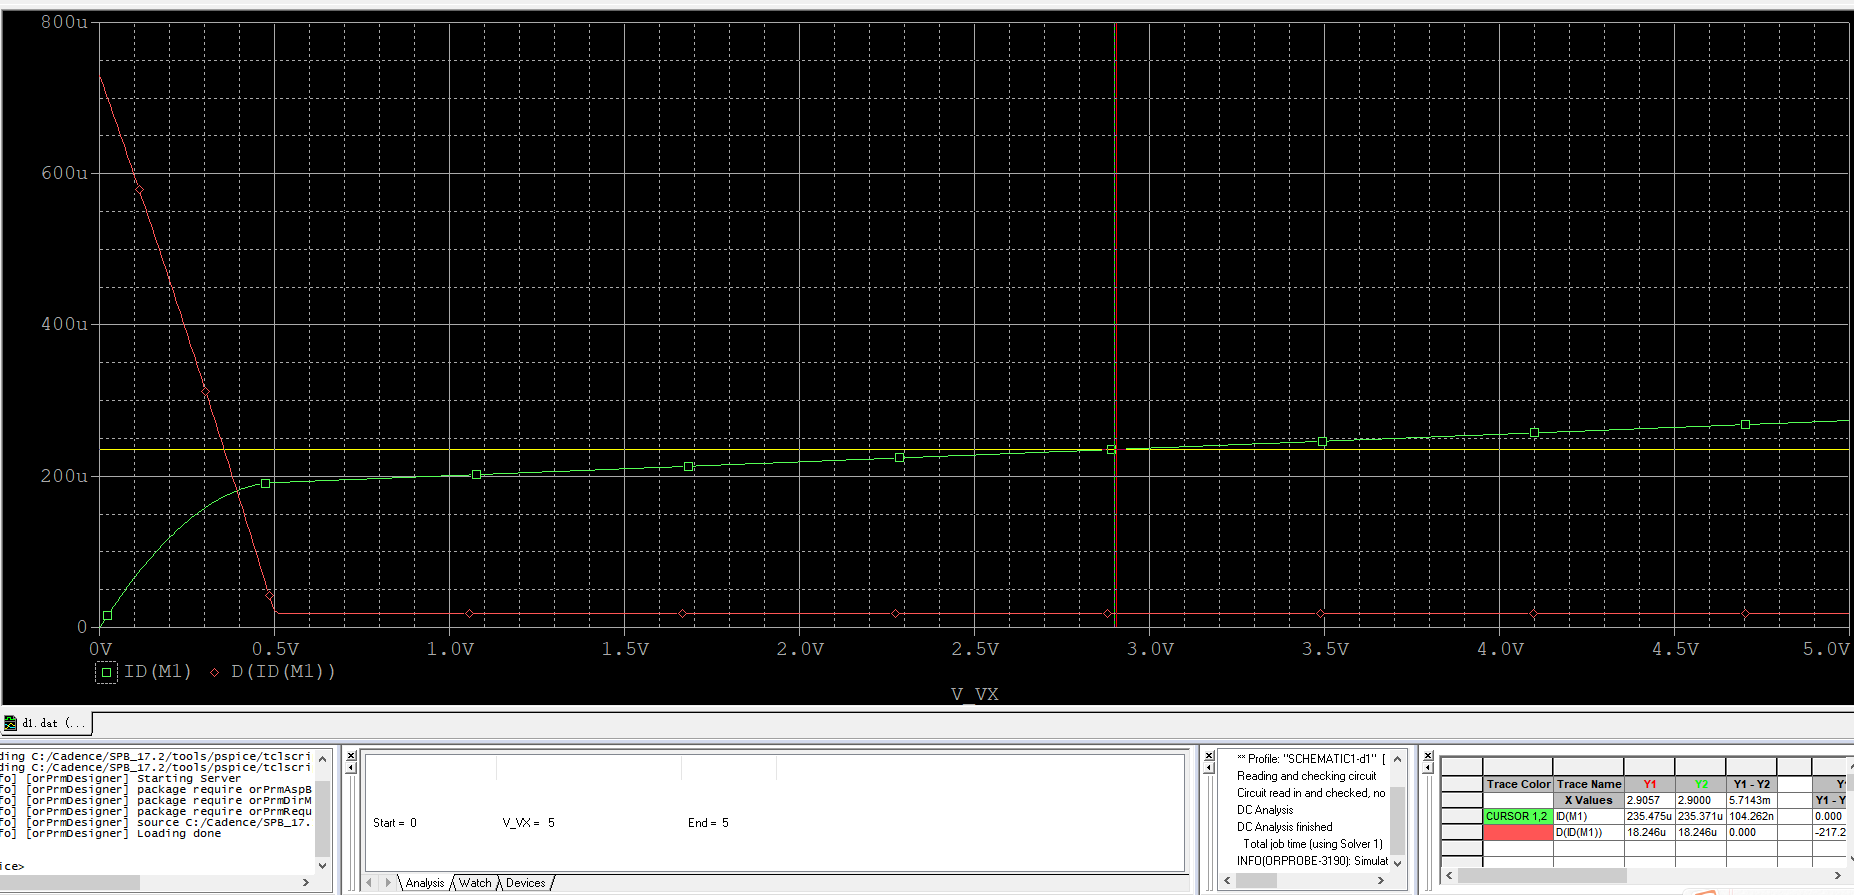
\includegraphics[scale=0.25]{P1.png}
\end{figure}
The voltage for saturation is about 5V and the output impedance is $\frac{1}{18.246\times10^{-6}}=54806\Omega$, which is very close to my calculated value.
\subsection{(ii)}
\begin{figure}[H]
\centering
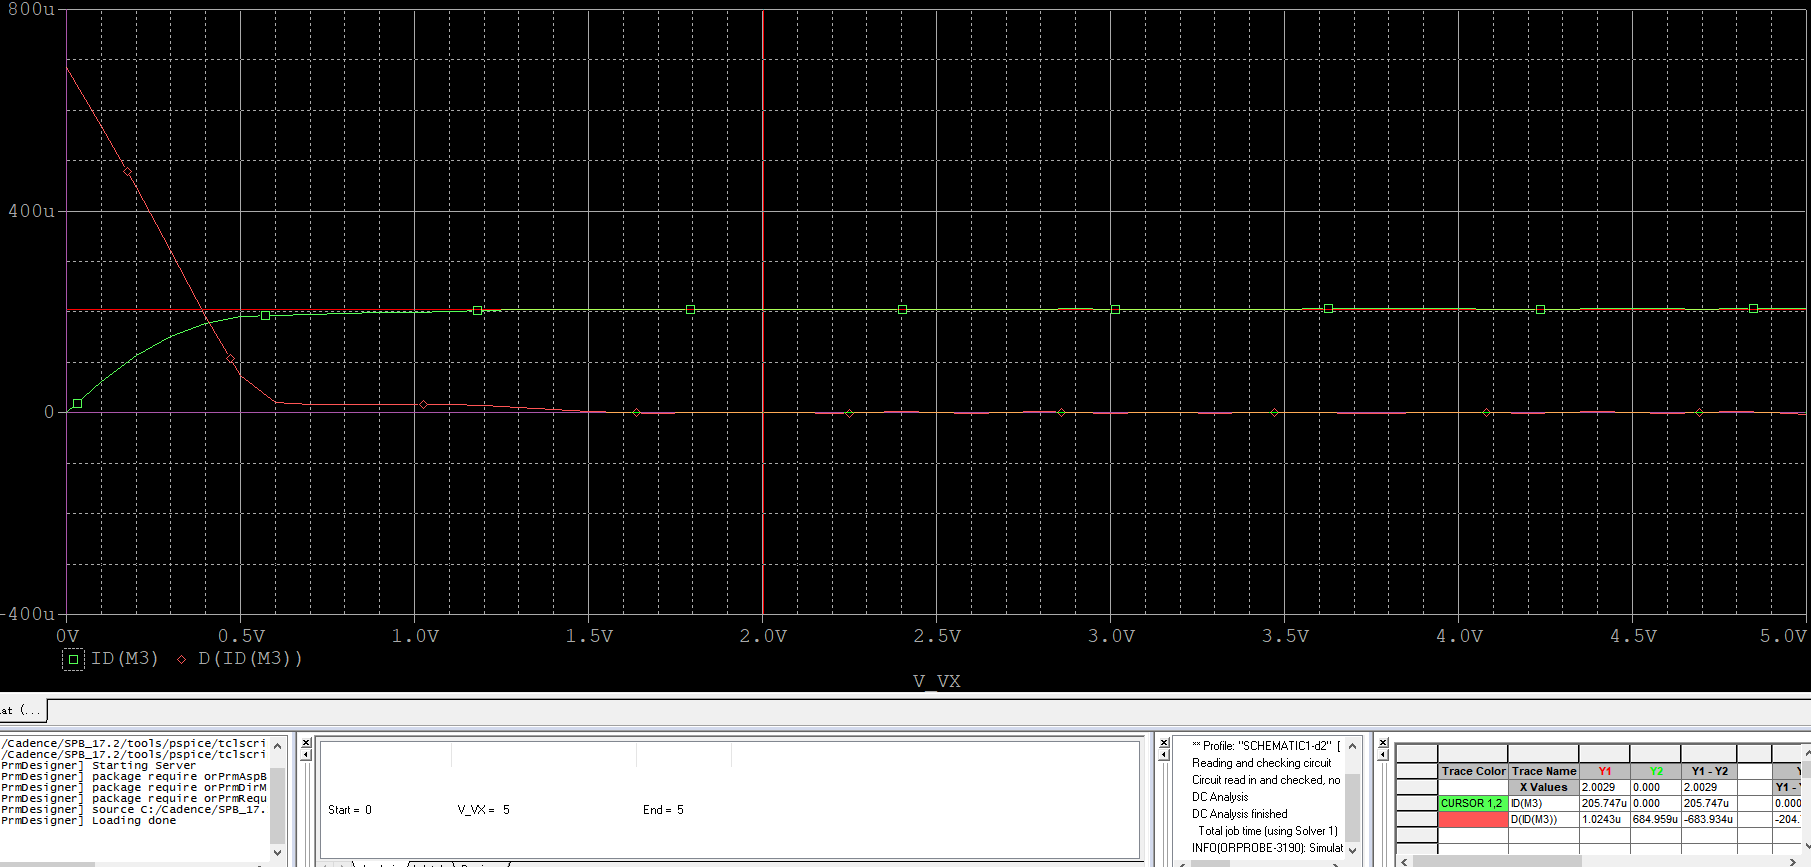
\includegraphics[scale=0.25]{P2.png}
\end{figure}
The voltage for saturation is about $1.5V$ and the output impedance is $\frac{1}{1.024\times10^{-6}}=976562\Omega$, which is very much smaller than my calculated value.
\end{document}